\documentclass[sigconf,screen,9pt]{acmart}

% Flag to disable all editing macros and make the document ready for
%  submission.
\newif\ifEditMode

% Editing mode.
\EditModetrue
% % Submission mode.
% % The `submission' mode merges certain comments and edits, and removes some
% % other notes, TODOs and remarks. For more details, refer to the `reviewing
% % macros' in the `vusec.sty' file.
% \EditModefalse


\usepackage{vusec}
\usepackage{frontmatter}
\usepackage{aliases}


\begin{document}


%% Thesis title.
\newcommand{\thesistitle}{My Thesis: what, why, and how?}


%% Author information.
%% (Used in a couple of places, so it's better to define them in one place.)
\newcommand{\thauthor}{Anonymous Penguin}
%%  Student number.
\newcommand{\thauthorid}{007}
\newcommand{\thauthoremail}{anonpenguin@student.vu.nl}
\newcommand{\thauthoraff}{Vrije Universiteit Amsterdam}


%% Thesis type.
%% Valid values are `vubachelor', `csmaster', `pdcsmaster', `csecmaster', and `litstudy'.
%%
\thtype{csecmaster}

%% Course code.
\thcc{XM\_0123}

%% Thesis title.
\thtitle{\thesistitle}

%% Paper/thesis author.
\thauthname{\thauthor}
\thauthid{\thauthorid}

%% First supervisor.
\thsvfirst{First supervisor's name}{First supervisor's title}

%% Daily supervisor.
\thsvdaily{Daily supervisor's name}{Daily supervisor's title}

%% Second reader.
\thrdrsecond{Second reader's name}{Second reader's title}

\pagenumbering{gobble}
%% Attach customize front matter.
\addfrontmatter{}


\title{\thesistitle}

\author{\thauthor}
\affiliation{
  \institution{\thauthoraff}
  \city{Amsterdam}
  \country{NL}
}
\email{\thauthoremail}


\begin{abstract}
\TODO{
This first and short section includes a summary of the work. A strong abstract
highlights the research problem, which the thesis addresses, succinctly
describes why the problem is worth pursuing, and highlights the contributions of
the thesis towards addressing the problem.
}


\lipsum[5]


%%% Local Variables:
%%% mode: latex
%%% TeX-master: "../thesis"
%%% End:

\end{abstract}

\maketitle

\pagenumbering{arabic}

\section{Introduction}\label{s:intro}

\stress{Think before you write, be careful how you write, and take feedbacks
seriously}~\cite{Heiser-WebArticle2022}.


This section includes some motivations behind the work, explicitly or implicitly
highlights the research question, provides a high-level explanation of the
solution, and describes the contributions.

\textcolor{lightgray}{\lipsum[1]}

\parai{Makefile.}
%
It is typical to build a PDF from the \LaTeX{} sources using \texttt{make}, but
resist the temptation to fill the \texttt{Makefile} with complex and unnecessary
rules or recipes.
%
You only need one line, where you invoke \texttt{latexmk}.
%
This template should also come bundled with a \texttt{Makefile}, which should
suffice in virtually all scenarios.

\textcolor{lightgray}{\lipsum[3-4]}

\begin{figure}[tbh]
    %% The macro `\onecolgrid' is defined in `vusec.sty'
    %% NOTE: The suffix "./figs/" is implicitly included for this relative path.
    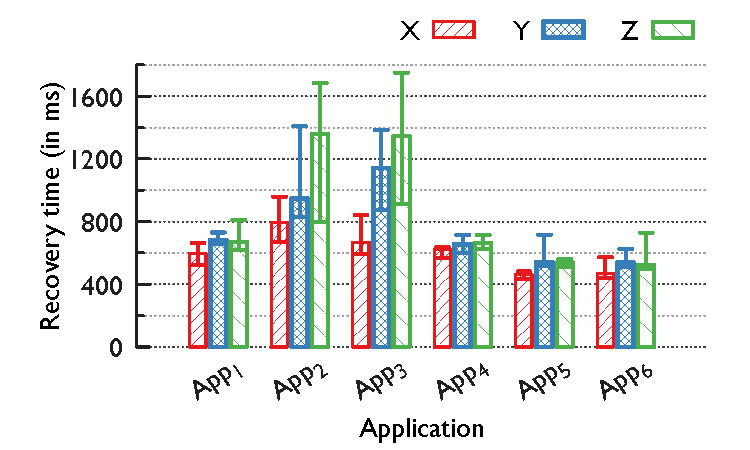
\includegraphics[width=\onecolgrid]{cache-by-app}
    %% Labels should immediately follow caption, to keep latex quiet.
    \figcap{Simple one-column figure. Please include a brief explanation or
    takeaway.}\label{fig:1col}
\end{figure}

\parai{Figures.}
%
Do not include figures that you do not refer to or discuss in the text.
%
Generate high-quality figures (Fig.~\ref{fig:1col})---think PDF or EPS.
%
With the number of tools and libraries that are available today for generating
beautiful plots, there is no excuse for producing ugly plots.
%
Figure caption must go at the bottom of a figure (Fig.~\ref{fig:3col}), and it
is also a good place to highlight the key takeaway of that figure.
%
Avoid using the position parameters `p' and `!', unless you are absolutely sure
that is exactly what you want.

\begin{figure*}[th]
    %% The macro `\threecolgrid' is defined in `vusec.sty'
    \begin{subfigure}[t]{\threecolgrid}
        %% NOTE: The suffix "./figs/" is implicitly included for these relative paths.
        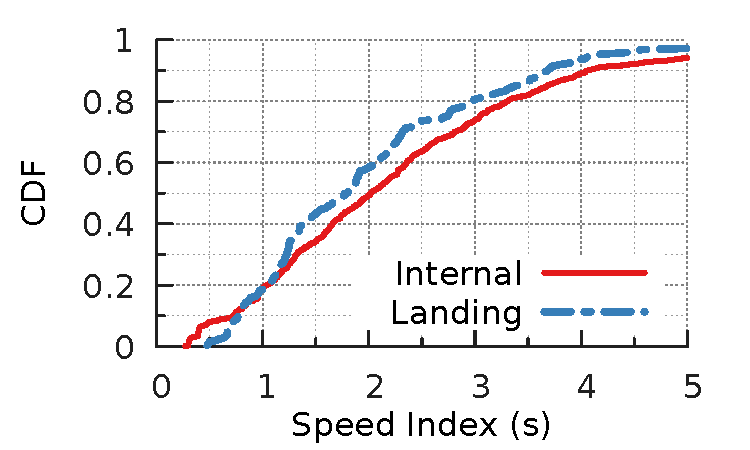
\includegraphics[width=\linewidth]{three-col/speed_index}
        \sfigcap{}\label{fig:3col-a}
    \end{subfigure}
    \begin{subfigure}[t]{\threecolgrid}
        %% NOTE: You do not have to mention the extension.
        %% (The example figures are in PDF format.)
        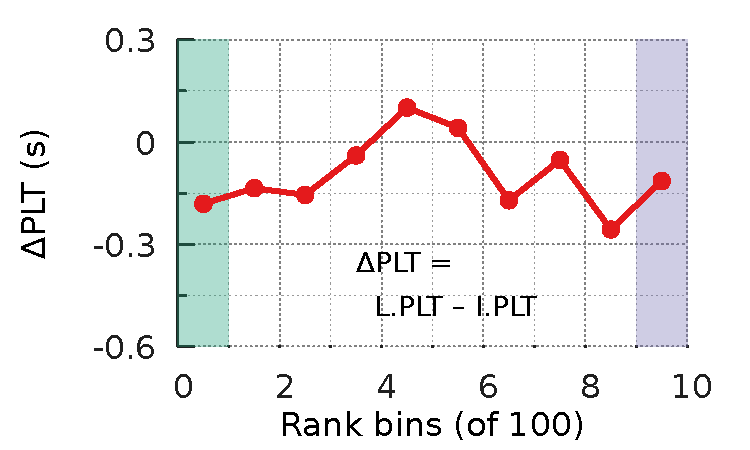
\includegraphics[width=\linewidth]{three-col/plt_ranks_diff}
        \sfigcap{}\label{fig:3col-b}
    \end{subfigure}
    \begin{subfigure}[t]{\threecolgrid}
        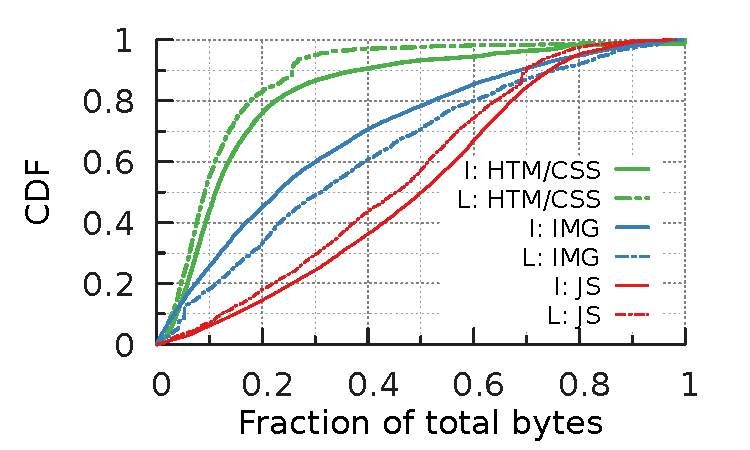
\includegraphics[width=\linewidth]{three-col/mimes}
        \sfigcap{}\label{fig:3col-c}
    \end{subfigure}
    %% Labels should immediately follow caption, to keep latex quiet.
    \figcap{Generate clear and beautiful figures (in PDF) that can be rendered side by side while still being easy to read and interpret. Choose colors wisely from the colorbrewer2.org website.}\label{fig:3col}
\end{figure*}

\textcolor{lightgray}{\lipsum[6-7]}

\begin{table}[tb]
    \centering
    \tabcap{A simple table describing the characteristics of a data set or the
    results of an experiment.}\label{tab:sample}
    \taburulecolor{black!45}
    \begin{tabu}{c|c|r|r|r|r}
        \toprule
        \multirow{2}{*}{\thead{Char.}} &
            \multirow{2}{*}{\thead{\#samples}} &
            \thead{Count} &
            \multicolumn{3}{c}{\thead{Perf. Score}}\\
        &
            &
            \thead{of items} &
            \thead{X} & \thead{Y} & \thead{Z} \\
        \midrule
        \stress{P}
            & 214 & 56 & 9 & 23 & 24 \\
        \stress{Q}
            & 117 & 27 & 7 & 10 & 10 \\
        \stress{R}
            & 222 & 11 & 6 & 4 & 1 \\
        \stress{S}
            & 187 &  9 & 1 & 6 & 2 \\
        \stress{T}
            & 180 & 16 & 7 & 5 & 4 \\
        \bottomrule
    \end{tabu}

\end{table}

\parai{Tables.}
%
The caption must go at the top of the table (Tab.~\ref{tab:sample}).
%
Do not use \texttt{\textbackslash{}hrule}.
%
Use \texttt{\textbackslash{}toprule} above the heading,
\texttt{\textbackslash{}midrule} below the heading, and
\texttt{\textbackslash{}bottomrule} below the last row.
%
You could also use \texttt{\textbackslash{}hrule} as a row separator.
%
Right align numerical values, and use math-mode for (large) numerical values to
force \LaTeX{} to use monospaced fonts and ensure right-alignment functions as
expected.

\textcolor{lightgray}{\lipsum[12-14]}

We summarize our contributions as follows.

\case{}
%
\textcolor{lightgray}{\lipsum[10][2-4]}

\case{}
% 
\textcolor{lightgray}{\lipsum[11][4-8]}

\case{}
% 
\textcolor{lightgray}{\lipsum[12][2-6]}

\case{}
% 
\textcolor{lightgray}{\lipsum[16][4-8]}

Depending on your degree program and/or supervisor, you may need to furnish the
“Artifact Appendix” (\S\ref{s:appendix}).


%%% Local Variables:
%%% mode: latex
%%% TeX-master: "../thesis"
%%% End:

\section{Background}\label{s:background}

This section provides the necessary context to help the reader understand the
remainder of the thesis.


\textcolor{lightgray}{\lipsum[16-20]}


%%% Local Variables:
%%% mode: latex
%%% TeX-master: "../thesis"
%%% End:

\section{Threat Model}\label{s:threat-model}

Use this section to address key questions: (a) What does this thesis or paper
assume about the attackers’ goals and objectives? (b) What do you assume about
the systems and their environment, etc.

\textcolor{lightgray}{\lipsum[7-11]}


%%% Local Variables:
%%% mode: latex
%%% TeX-master: "../thesis"
%%% End:

\section{Overview}\label{s:overview}


\TODO{
This section provides a high-level outline of the proposed system or solution.
It typically illustrates the system architecture or the interactions between the
different solution components (via a “boxes-and-arrows” diagram) from a user’s
perspective.
}


\lipsum[1-6]


%%% Local Variables:
%%% mode: latex
%%% TeX-master: "../thesis"
%%% End:

\section{Design}\label{s:design}

In this section, you would provide a high-level description of the system or
solution and explain your design choices.

\textcolor{lightgray}{\lipsum[22-36]}


%%% Local Variables:
%%% mode: latex
%%% TeX-master: "../thesis"
%%% End:

\section{Evaluation}\label{s:evaluation}

Discuss the design of your experiments, the results you obtained, and how they
help in evaluating the claims you made in the introduction. You may also use the
evaluation results in this section to justify your design choices or assess the
contributions of different aspects  of your design towards the overall goals.

\textcolor{lightgray}{\lipsum[12-28]}


%%% Local Variables:
%%% mode: latex
%%% TeX-master: "../thesis"
%%% End:

\section{Discussion}\label{s:discussion}

A “limitations” section, as the name implies, describes scenarios where the
proposed solution may not work well. Although a “discussion” section could also
highlight limitations of the proposed work, it focuses on analyzing the
implications of the proposed work for current and future research.


\textcolor{lightgray}{\lipsum[26-32]}


%%% Local Variables:
%%% mode: latex
%%% TeX-master: "../thesis"
%%% End:

\section{Related Work}\label{s:related}


\TODO{
It is quite unlikely that you were the first to address this problem. Please use
this section, hence, to discuss what prior work had done and how your solution
is different from or better than prior work. You may place this section
immediately after the “Background” section, if necessary.
}


\lipsum[14-17][4-8]


\TODO{
Srinivasan Keshav's old---but still relevant---article on how to read a paper is an
excellent read in general for performing literature
surveys~\cite{Keshav-SIGCOMMCCR2007}.
}


%%% Local Variables:
%%% mode: latex
%%% TeX-master: "../thesis"
%%% End:

\section{Conclusion}\label{s:conclusion}

Briefly summarize your contributions, and share a glimpse of the implications of
this work for future research.

\textcolor{lightgray}{\lipsum[12-13]}


%%% Local Variables:
%%% mode: latex
%%% TeX-master: "../thesis"
%%% End:


\bibliographystyle{ACM-Reference-Format}
\bibliography{references}

\clearpage
\appendix
\section{Artifact Appendix}\label{s:appendix}

The instructions below on how to furnish this section are based on the USENIX
Security ’22 Artifact Appendix Guidelines~\cite{USENIX-WebArticle2022}.

\subsection{Abstract}

Describe the artifacts that you produced as part of this thesis. Describe
briefly how they support this thesis.
%
They include, but not limited to, implementations of a system or solution
described in the thesis, tools for evaluating certain contributions of this
thesis, software or hardware for gathering measurements, and software for
generating the visualizations used in the study.


%%% Local Variables:
%%% mode: latex
%%% TeX-master: "../thesis"
%%% End:

\subsection{Checklist}

This mandatory section provides a quick overview of the requirements for a
reader to evaluate or reuse the artifact(s) produced as part of your thesis.
%
Please approach your advisor if you have questions such as what constitutes an
artifact, how to make them accessible, and what level of detail to provide to
allow reuse of such artifacts.
%
We have provided a extensive checklist of items that are applicable to a broad
range of projects.
%
Remove items that are not relevant to your artifact(s); otherwise, simply
replace the description of each item, with details relevant to your artifact.
%
Leave the formatting intact.

\chk{Algorithm}:
%
If you are presenting a new algorithm, succinctly describe it along with 1-2 key
insights.

\chk{Benchmark}:
%
Describe any benchmarks (e.g., PARSEC, LINPACK, and SPEC) that you used in your
thesis and their sizes.
%
Explain how to access them.
%
If the benchmark is private, indicate whether it has a public analog.

\chk{Compilation}:
%
If your artifact requires a specific compiler, mention which compiler, what
version, and whether it is public.

\chk{Transformations}:
%
If your artifact uses a program transformation tool (source-to-source,
binary-to-binary, compiler pass, etc.), mention the tool, version, and whether
it is public.

\chk{Binary}:
%
Indicate whether your artifact(s) includes binaries, and, if it does, mention
their versions and if they are OS specific.

\chk{Model}:
%
Describe specific models (e.g., ImageNet, AlexNet, and MobileNets) used in your
thesis, their sizes, and how to access them.

\chk{Data set}:
%
Identify if your thesis uses any specific data sets, and briefly characterize
these data sets, and explain how to access them.

\chk{Run-time environment}:
%
Clarify whether your artifact is OS-specific (Linux, Windows, MacOS, Android,
etc.), and, if yes, list the version, (key) software dependencies (JIT, libs,
run-time adaptation frameworks, etc.), and whether the artifact requires
root (or administrator) privileges?

\chk{Hardware}:
%
Describe whether your thesis has specific hardware requirements (e.g.,
supercomputer, architecture simulator, GPU, and FPGA) or specific features
(e.g., hardware counters for measuring power consumption and root-level access
to CPU or GPU frequency).

\chk{Run-time state}:
%
Explain whether the evaluation of your artifact is sensitive to run-time state
(e.g., cold or hot cache, and network or cache contentions).

\chk{Execution}:
%
List any specific (environment) conditions (e.g., sole user, process pinning,
profiling, and adaptation) required by your artifact for any experiment, and
also how long it takes for the experiments (or executions) to run or finish.

\chk{Security, privacy, and ethical concerns}:
%
Highlight any specific security, privacy, or ethical concerns with running the
experiments (e.g., malware sample sandboxing and network scanning).

\chk{Metrics}:
%
Describe the metrics you report (e.g., execution time and inference per second)
in your experiments.

\chk{Output}:
%
Briefly explain the results generated in various experiments and their formats
(e.g., console, file, table, graph).
%
Indicate whether the expected results are included as part of the artifact(s).

\chk{Experiments}:
%
Explain how to prepare the environment for running experiments, replicate or
reproduce the results (for instance, explain the OS scripts to run, manual steps
to be taken by the user, etc.)?
%
We strongly recommend you to emphasize the \textit{maximum allowable variation}
in the (empirical) results.

\chk{Approximate disk space}:
%
Mention the storage requirements for the artifact and its experiments, so that
the people attempting to re-use or re-evaluate the artifact can provision their
environments appropriately.

\chk{Approximate preparation time}:
%
Emphasize how long it would take to prepare the environment and artifact before
anyone can run the experiments to reproduce the results.

\chk{Approximate time to complete experiments}:
%
Clarify how long it would take for a user to complete all experiments from start
to finish, excluding the preparation time.

\chk{Public availability}:
%
If your artifact is or will be publicly available, provide the reference or
location to access it, along with version and other metadata to fetch the exact
copy of the artifact used in this thesis.

\chk{Code license(s)}:
%
If your artifact will be publicly available, mention licenses, if any,
associated with one or more components of your artifact.

\chk{Data license(s)}:
%
If your artifact will be publicly available, mention licenses, if any, for the
data sets you used in your artifact(s).

\chk{Workflow framework(s)}:
%
Mention whether any workflow framework was (or could be) used for automating and
customizing the experiments.

\chk{Archive}:
%
If you are artifacts are archived on a publicly accessible portal, mention its
DOI, or stable reference.
%
If you archived the artifact(s) in a public versioning system (e.g., GitHub), which can evolve over
time, provide a (stable) reference (e.g., a URL pointing to the commit hash or
tag) to the version used in this thesis.


%%% Local Variables:
%%% mode: latex
%%% TeX-master: "../thesis"
%%% End:

\subsection{Reproducibility}

In this mandatory section, describe the procedures to setup the environment for
evaluating or reusing your artifact(s).
%
The descriptions should be targeted at being accessible to novice users.

\paraib{Accessing the artifact(s)}
%
Describe how a reader can access your artifact(s).
%
If they are publicly available in a repository, provide the URL and clear
instructions (targeted at a novice user) on how to download an exact replica of
the artifact described in this appendix.
%
Suppose that the artifact is private, provide guidelines on how a reader could
approach relevant people (i.e., the author of this thesis or supervisors
involved in this project) to obtain access.

\paraib{Installation and configuration}
%
Describe how a (novice) user can install the artifact on their system or
platform.
%
Highlight the various hardware and software dependencies, and, explain in
detail, wherever applicable, how the user could install or configure these
dependencies.

\paraib{Experiment Workflow}
%
Provide a high-level overview of the (experiment) workflow, shedding light on
how you implemented it, how users can set it up and invoke it, and (optionally)
how they can customize or extend it.

\paraib{Evaluation and Expected Result}
%
Enumerate the key claims of your thesis and describe which experiment and result
supports that claim.
%
Explain, in detail, all the steps to reproduce each of these key results.
%
Where applicable, explain the maximum variation that is permissible in these
results.

\paraib{Experiment Customization}
%
If possible, and relevant, describe how to customize your workflow (e.g., to use
a different data set, benchmark, model, application, and environment).
%
If customizations are irrelevant to the artifact(s) produced in this thesis,
please remove this paragraph.


%%% Local Variables:
%%% mode: latex
%%% TeX-master: "../thesis"
%%% End:



%%% Local Variables:
%%% mode: latex
%%% TeX-master: "../thesis"
%%% End:


\end{document}


%%% Local Variables:
%%% mode: latex
%%% TeX-master: t
%%% End:
